\section{Quasi-Convexity and Weak Lower Semicontinuity}
We show that quasi-convexity of $f$ is both necessary and sufficient for weak lower semicontinuity. Recall that $f:\mathbb{R}^{m\times d}\longrightarrow\mathbb{R}_\infty$ is quasi-convex if for all $A\in\mathbb{R}^{m\times d}$, all $\psi\in C_c^\infty(B_1(0);\mathbb{R}^m)$
\[\int_{B_1(0)}{f(A+\nabla\psi(x))\mathrm{d}x}\geq\vol{B_1(0)}f(A).\]
According to \hyperlink{remark_4_1_5}{Remark 4.1.5 (b)}, we can even consider $\psi\in W_0^{1,\infty}(B_1(0);\mathbb{R}^m)$ and replace the unit ball $B_1(0)$ with every arbitrary bounded, open set $D\subset\mathbb{R}^d$.\\

\begin{theorem}[Vitali covering]
Let $\Omega\subset\mathbb{R}^d$ be bounded and open. Fix $\delta>0$. Then there exists a countable family $\mathcal{G}$ of pairwise disjoint closed balls in $\Omega$ such that $\diam{B}\leq\delta$ for each $B\in\mathcal{G}$ and $\mathcal{L}^d(\Omega\setminus\bigcup_{B\in\mathcal{G}}{B})=0$.
\end{theorem}
\textit{Proof:}\\
\cite[Kapitel V, §1 Produktma{\ss}e, 5. Das $p$-dimensionale \"au{\ss}ere Hausdorff-Ma{\ss}, Satz 1.14]{Elst1996MIT}.\hfill$\blacksquare$\\[11pt]

\begin{theorem}[Quasi-convexity is necessary and sufficient]
Let $\Omega\subset\mathbb{R}^d$ be a bounded, open Lipschitz domain. Fix $p\in(1,\infty)$. Let $f:\mathbb{R}^{m\times d}\longrightarrow[0,\infty)$ be continuous such that $f(A)\leq C(1+\lvert A\rvert^p)$ for all $A\in\mathbb{R}^{m\times d}$ and some $C>0$. Consider
\[I:W^{1,p}(\Omega;\mathbb{R}^m)\longrightarrow[0,\infty),\qquad I(u):=\int_\Omega{f(\nabla u(x))\mathrm{d}x}.\]
Then, the following assertions are equivalent:
\begin{itemize}
	\item[(a)] $I$ is weakly sequentially lower semicontinuous on $W^{1,p}(\Omega;\mathbb{R}^m)$.
	\item[(b)] $f$ is quasi-convex.\\
\end{itemize}
\end{theorem}
\textit{Remark: The lower bound of $f$ by zero is a relatively strong assumption. But a lower bound of polynomial type of order $p$ would not work, if we e.g. consider the example of Tartar, $m=d=2$ and $f(A)=\det(A)$, then this is poly-convex, hence quasi-convex, and fulfills $\lvert f(A)\rvert\leq c\lvert A\rvert^2$, but its associated functional is not weakly lower semicontinuous on $H^1((0,1)^2;\mathbb{R}^2)$.}\\

\textit{However, a lower bound of the type $f(A)\geq c_1\lvert A\rvert^{p-\varepsilon}-c_2$ for $\varepsilon>0$ would be enough to prove the equivalence, see \cite[Part II, Chapter 8, Section 8.2 Weak lower semicontinuity, 8.2.4 Lower semicontinuity for general quasiconvex functions for $1\leq p<\infty$]{Daco2007DMCV}.}

\textit{Proof:}
\begin{itemize}
	\item[(a)] $\Rightarrow$ (b): Assume $I$ is weakly lower semicontinuous. There exist $x\in\mathbb{R}^d$ and $R>0$ such that $B_1(0)\subset\mathrel\subset\Omega':=y+R\Omega$, and $I$ remains weakly sequentially lower semicontinuous on $W^{1,p}(\Omega';\mathbb{R}^m)$. That means, after eventual rescaling and translation, we can assume $B_1(0)\subset\mathrel\subset\Omega$. Let $A\in\mathbb{R}^{m\times d}$, $\psi\in C_c^\infty(B_1(0);\mathbb{R}^m)$. We need to show
	\[f(A)\leq\frac{1}{\vol{B_1(0)}}\int_{B_1(0)}{f(A+\nabla\psi(x))\mathrm{d}x}.\]
	For $j\in\mathbb{N}$ consider a Vitali covering of $B_1(0)$, that means, by \hyperlink{theorem_4_3_1}{Theorem 4.3.1} we can find $r_k^{(j)}\in(0,\delta_j)$, $x_k^{(j)}\in B_1(0)$, where $\delta_j:=\frac{1}{j}$, such that
	\[B_1(0)=\dot\bigcup_{k\in\mathbb{N}}{B_{r_k^{(j)}}(x_k^{(j)})}\cup N\]
	for some $N\subset B_1(0)$ with $\mathcal{L}^d(N)=0$. Define for $j\in\mathbb{N}$ the function $u_j:\Omega\longrightarrow\mathbb{R}^m$ via
	\[u_j(x):=Ax+\left\{\begin{array}{rl}
		r_k^{(j)}\psi\left(\frac{x-x_k^{(j)}}{r_k^{(j)}}\right)&\text{if }x\in B_{r_k^{(j)}}(x_k^{(j)}),\\
		0&\text{otherwise}
	\end{array}\right.\]
	so $u_j$ just consists of scaled copies of $\psi$, where each copy is living on one of the balls $B_{r_k^{(j)}}(x_k^{(j)})$. Clearly we have $u_j\to u_*$ in $L^p(\Omega;\mathbb{R}^m)$ with $u_*(x)=Ax$, since $\psi$ is bounded and $\sup\{r_k^{(j)}\mid k\in\mathbb{N}\}\to0$ for $j\to\infty$. Furthermore, $\nabla u_j\rightharpoonup A=\nabla u_*$ in $L^p(\Omega;\mathbb{R}^{\times d})$ because $\rVert\nabla u_j\rVert_{L^\infty(\Omega)}$ is bounded uniformly in $j$, $W^{1,p}(\Omega;\mathbb{R}^{m\times d})$ is reflexive and embeds into $L^p(\Omega;\mathbb{R}^m)$. By assumption we have
	\[\vol{\Omega}f(A)=I(u_*)\leq\liminf_{j\to\infty}{\int_\Omega{f(\nabla u_j(x))\mathrm{d}x}}.\]
	Use that $\nabla u_j=A$ in $\Omega\setminus B_1(0)$. Hence we obtain
	\begin{align*}
		\vol{B_1(0)}f(A)&\leq\liminf_{j\to\infty}{\int_{B_1(0)}{f(\nabla u_j(x))\mathrm{d}x}}\\
		&=\liminf_{j\to\infty}{\sum_{k=1}^\infty{\int_{B_{r_k^{(j)}}(x_k^{(j)})}{f(A+\nabla\psi\left(\frac{x-x_k^{(j)}}{r_k^{(j)}}\right))\mathrm{d}x}}}\\
		&=\liminf_{j\to\infty}{\sum_{k=1}^\infty{(r_k^{(j)})^d\int_{B_1(0)}{f(A+\nabla\psi(y))\mathrm{d}y}}},
	\end{align*}
	where the second line follows since $f\geq0$, and the third is a change of variables. Since
	\[\vol{B_1(0)}=\sum_{k=1}^\infty{\vol{B_{r_k^{(j)}}(x_k^{(j)})}}=\sum_{k=1}^\infty{(r_k^{(j)})^d\vol{B_1(0)}}\]
	it follows that $\sum_{k=1}^\infty{(r_k^{(j)})^d}=1$. Therefore we have shown
	\[\vol{B_1(0)}f(A)\leq\int_{B_1(0)}{f(A+\nabla\psi(x))\mathrm{d}x}.\]\\

	For this implication, we haven't used the growth condition.
	\item[(b)] $\Rightarrow$ (a): Assume $f$ is quasi-convex. Since $f$ is continuous and satisfies the $p$-growth, and since $W_0^{1,\infty}(\Omega;\mathbb{R}^m)$ is dense in $W_0^{1,p}(\Omega;\mathbb{R}^m)$, we can use in the definition of quasi-convexity even test functions $\psi\in W_0^{1,p}(\Omega;\mathbb{R}^m)$.\\

	Let $(u_k)_{k\in\mathbb{N}}\subset W^{1,p}(\Omega;\mathbb{R}^m)$, $u\in W^{1,p}(\Omega;\mathbb{R}^m)$ such that $u_k\rightharpoonup u_*$ in $W^{1,p}(\Omega;\mathbb{R}^m)$ as $k\to\infty$. We are going to show $I(u_*)\leq\liminf_{k\to\infty}{I(u_k)}$ during three steps, gradually weaken the assumption on the given objects.\\

	\textit{Step 1:}
	\begin{itemize}
		\item[] Suppose first $u_*$ is affine, i.e. $\nabla u_*\equiv A$ for some constant matrix $A\in\mathbb{R}^{m\times d}$, and also that $u_k-u_*\in W_0^{1,p}(\Omega;\mathbb{R}^m)$. With these assumptions we estimate
		\[I(u_*)=\int_\Omega{f(A)\mathrm{d}x}=\vol{\Omega}f(A)\leq\int_\Omega{f(A+\nabla(u_k-u_*)(x))\mathrm{d}x}=I(u_k)\]
		for each $k\in\mathbb{N}$. Hence $I(u_*)\leq\liminf_{k\to\infty}{I(u_k)}$.\\
	\end{itemize}

	\textit{Step 2:}
	\begin{itemize}
		\item[] Now suppose that $u_*$ is affine, but the $u_k-u_*$ do no longer need to be in $W_0^{1,p}(\Omega;\mathbb{R}^m)$. Let $\Omega_0\subset\mathrel\subset\Omega$ and $R:=\frac{1}{2}\operatorname{dist}(\Omega_0,\partial\Omega)>0$. For all $N\in\mathbb{N}$, all $n=1,\dotsc,N$, set
		\[\Omega_n=\left\{x\in\Omega\,\middle\vert\,\operatorname{dist}(x,\Omega_0)<\frac{n}{N}R\right\}.\]
		Then $\Omega_0\subset\Omega_1\subset\dotsc\subset\Omega_N\subset\Omega$.

		\begin{figure}[ht]
			\centering
			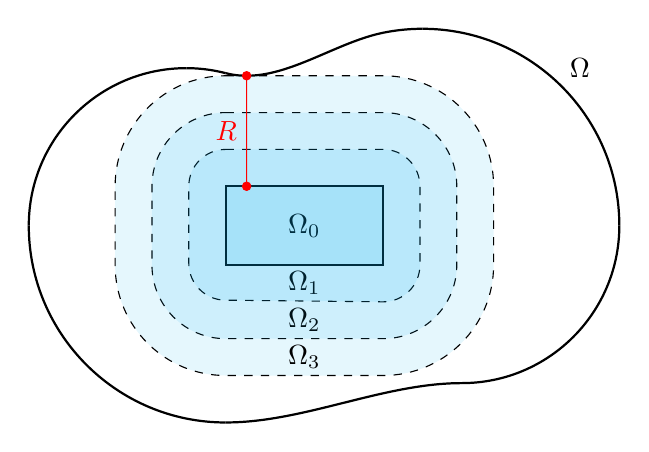
\begin{tikzpicture}
				% Shape of Omega
				\node at (3.5, 2) {$\Omega$};
				\draw[thick] (-3.5, 0) arc (180:90:2);
				\draw[thick] plot[smooth, domain=-1.5:-1] (\x, {sqrt(4-(\x+1.5)^2)});
				\draw[thick] plot[smooth, domain=-1:1] (\x, {-0.14177*(\x)^3+0.11558*(\x)^2+0.39827*\x+2.07741});
				\draw[thick] plot[smooth, domain=1:1.5] (\x, {sqrt(6.25-(\x-1.5)^2)});
				\draw[thick] (4, 0) arc (0:90:2.5);
				\draw[thick] (4, 0) arc (360:270:2);
				\draw[thick] plot[smooth, domain=-1.5:1.5] (\x+0.5,{-0.03704*(\x)^3+0.25*\x-2.25});
				\draw[thick] (-3.5, 0) arc (180:270:2.5);

				% Omega_0
				\draw[thick, fill=cyan, fill opacity=0.1] (-1, -0.5) rectangle (1, 0.5);
				\node at (0, 0) {$\Omega_0$};

				% Omega_1
				\draw[dashed, fill=cyan, fill opacity=0.1] (-1, 0.9678) -- (1, 0.9678) arc (90:0:0.4678) --(1.4678, -0.5) arc (360:270:0.4678) -- (-1, -0.94678) arc (270:180:0.4678) -- (-1.4678, 0.5) arc (180:90:0.4678);
				\node at (0, -0.7339) {$\Omega_1$};

				% Omega_2
				\draw[dashed, fill=cyan, fill opacity=0.1] (-1, 1.4356) -- (1, 1.4356) arc (90:0:0.9356) --(1.9356, -0.5) arc (360:270:0.9356) -- (-1, -1.4356) arc (270:180:0.9356) -- (-1.9356, 0.5) arc (180:90:0.9356);\node at (0, -1.2017) {$\Omega_2$};

				% Omega_3
				\draw[dashed, fill=cyan, fill opacity=0.1] (-1, 1.9034) -- (1, 1.9034) arc (90:0:1.4034) --(2.4034, -0.5) arc (360:270:1.4034) -- (-1, -1.9034) arc (270:180:1.4034) -- (-2.4034, 0.5) arc (180:90:1.4034);\node at (0, -1.6695) {$\Omega_3$};

				% Radius R
				\draw[red, fill=red] (-0.73337, 0.5) circle (1.5pt) -- node[left] {$R$} (-0.73337, 1.90341) circle (1.5pt);
			\end{tikzpicture}
			\caption{Illustration of the situation with $\Omega_0\subset\dotsc\subset\Omega_3\subset\Omega$.}
		\end{figure}

		For $n=1,\dotsc,N$ consider $\varphi_n\in C^\infty(\Omega)$ with $0\leq\varphi_n\leq 1$, $\varphi_n\equiv1$ in $\Omega_{n-1}$, $\varphi_n\equiv0$ in $\Omega\setminus\Omega_n$ and $\lvert\nabla\varphi_n\rvert\leq\frac{2N}{R}$ in $\Omega$. (Such $\varphi_n$ can be constructed by mollifying certain distance functions.) Set $v_k^{(n)}:=u_*+\varphi_n\cdot(u_k-u_*)$ and compute
		\[\nabla v_k^{(n)}=\left\{\begin{array}{rl}
			\nabla u_*\equiv A&\text{in }\Omega\setminus\Omega_n,\\
			\nabla u_k&\text{in }\Omega_{n-1},\\
			A+\varphi_n\nabla(u_k-u_*)+(u_k-u_*)\nabla\varphi_n&\text{in }\Omega_n\setminus\Omega_{n-1}.
		\end{array}\right.\]
		Then $v_k^{(n)}-u_*\in W_0^{1,p}(\Omega;\mathbb{R}^m)$ and hence quasi-convexity gives
		\begin{align*}
			I(u_*)&\leq\int_\Omega{f\left(A+\nabla(v_k^{(n)}-u_*)(x)\right)\mathrm{d}x}\\
			&=\int_{\Omega_{n-1}}{f(\nabla u_k(x))\mathrm{d}x}+\int_{\Omega\setminus\Omega_n}{f(A)\mathrm{d}x}\\
			&\qquad\qquad+\int_{\Omega_n\setminus\Omega_{n-1}}{f\bigl(A+\varphi_n(x)\nabla(u_k-u_*)(x)+(u_k-u_*)(x)\nabla\varphi_n(x)\bigr)\mathrm{d}x}\\
			&\leq\int_\Omega{f(\nabla u_k(x))\mathrm{d}x}+C\int_{\Omega\setminus\Omega_0}{(1+\lvert A\rvert^p)\mathrm{d}x}\\
			&\qquad\qquad+\widetilde{C}\int_{\Omega_n\setminus\Omega_{n-1}}{\left(1+\lvert A\rvert^p+\lvert\nabla u_k(x)\rvert^p+\lvert(u_k-u_*)(x)\rvert^p\Bigl(\frac{N}{R}\Bigr)^p\right)\mathrm{d}x},
		\end{align*}
		where we have used in the last estimate that $f$ is non-negative and satisfies the $p$-growth, and that $0\leq\varphi_n\leq 1$. Now sum over $n\in\{1,\dotsc,N\}$ and divide by $N$ to get
		\begin{align*}
			I(u_*)&\leq\int_\Omega{f(\nabla u_k(x))\mathrm{d}x}+C\int_{\Omega\setminus\Omega_0}{(1+\lvert A\rvert^p)\mathrm{d}x}\\
			&\qquad\qquad+\frac{\widetilde{C}}{N}\int_{\Omega_N\setminus\Omega_0}{\left(1+\lvert A\rvert^p+\lvert\nabla u_k(x)\rvert^p+\lvert(u_k-u_*)(x)\rvert^p\Bigl(\frac{N}{R}\Bigr)^p\right)\mathrm{d}x}.
		\end{align*}
	\end{itemize}
\end{itemize}